\subsection{Frozen external UPR transfer feasibility}

A metadata-qualified local source extends the audit beyond the exposed development banks. Original Adamson UPR counts and full guide barcodes provide matched controls, three exact genetic singles and three pair identities in each of three chemical backgrounds \citep{adamson2016}. Publisher methods map capture groups to tunicamycin, thapsigargin and DMSO. The ATF6/PERK/IRE1 triple is genuine, but one triple identity supports inventory rather than a general higher-order benchmark. The backgrounds alias capture libraries, and independent culture initiation is unverified.

The fixed observed-single experiment aligns 10,423 genes using source-selected Norman genes and exact query Ensembl metadata. It freezes the Norman library normalizer and source-only three-fold selection over the existing mean, global, summed-single, pair-product and mixed menus. Source-selected global correction and mixed predictions are saved before evaluator access. All nine pair/background outcomes are scored once locally. This is a public-source feasibility pilot, not sealed, powered joint pair/state confirmation.

\begin{center}\small\begin{tabular}{lr}\toprule Model & MSE\\\midrule

additive & 0.00184324\\

mean residual & 0.00234538\\

global correction & 0.00292072\\

single sum & 0.00252739\\

pair product & 0.00289898\\

mixed & 0.00264696\\

\bottomrule\end{tabular}\end{center}

The frozen mixed candidate gains 9.37\% relative to the source-selected correction, with diagnostic paired MSE-reduction interval $[-0.00015503,0.00067825]$. Its lower bound includes zero, so the materiality gate fails. Additivity has MSE 0.00184324, lower than the source-selected correction's 0.00292072; a favorable mixed-versus-correction point estimate cannot establish value over this simpler retained competitor. No post-query family replacement or architecture advancement occurs.

Preparation takes 4.95 seconds with 3.08 GB process peak working set. Frozen source fitting takes 1.78 seconds with 370.0 MB completion RSS. Both use one CPU thread and remain below the registered budgets. The crossed target/background bootstrap retains 1773 nonempty draws from 2,000; it holds reference means and selection fixed and supplies no biological confidence interval. CRISPRa-to-CRISPRi, study and chemical/capture shifts remain confounded.

\begin{figure}[ht]\centering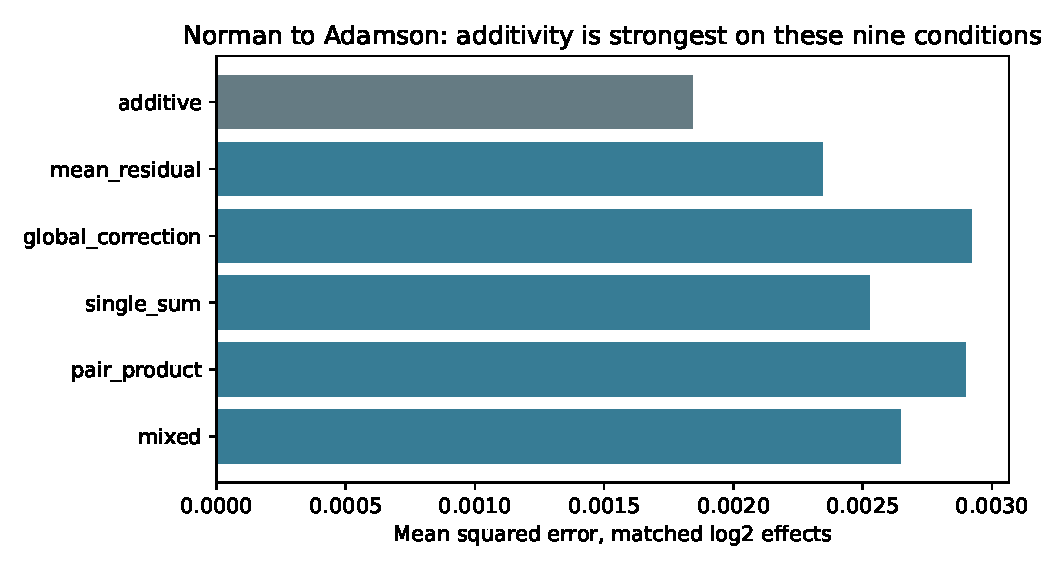
\includegraphics[width=.9\linewidth]{evidence/adamson_transfer_results.pdf}\caption{All retained competitors on the same nine external conditions. Additivity is stronger; the frozen mixed candidate fails the paired-uncertainty gate.}\end{figure}
